\chapter{Fuzzy Landing}\label{c:landing}
\section{Introduction}
With the ever-increasing proliferation of small unmanned air vehicles (sUAVs) and their use in commercial and
emergency response applications, there is a growing need for intelligent, reliable control methodologies to
safely manage their navigation, especially in possibly congested areas such as disaster areas or urban
centers. Commercial delivery companies are moving towards an automated model with reduced human operator
intervention to increase the efficiency of their deliveries. One such model consists of a vehicle-based sUAV
which departs from the delivery vehicle to make a delivery to a remote residence. Upon completing the
delivery, the sUAV returns to the vehicle and docks to receive additional packages. Considering the small
target size of a landing platform affixed to the vehicle, and the highly dynamic conditions in which
deliveries may be accomplished, the control effort must be accurate and robust in the face of disturbances.

Fuzzy control is able to accommodate nonlinearities in the dynamic system such as are found in the situation
of an air vehicle to ground transport rendezvous\cite{Ionita_2005}. Current approaches for
developing trajectory paths have focused on time-optimality\cite{Adams_2012}\cite{Hehn_2012} and not
necessarily on lightweight, on-board controllers. In contrast, this work will optimize for reduced control
effort and computational simplicity and efficiency. The control developed in this will be largely agnostic to
the large linearities inherent in the system dynamics and will apply linguistic variables and logic to
intuitively attain the interception and landing. Accuracy will be paramount as the target platform is nearly
equally-sized to the sUAV.

\section{System Architecture}
The research setup consists of a quadrotor aircraft of size \SI{450}{\mm} on the diagonal and a mobile rover
robot with a \SI{255}{mm} radius landing platform affixed to it (as shown in \cref{f:lezl-olli}. The quadrotor
is controlled by a Pixhawk flight controller which uses the PX4 flight control firmware. This flight
controller allows for an on-board computer to take over control of the aircraft via a serial wire connection.
A small Linux-based computer is placed on the quadrotor which sends velocity setpoints to the flight
controller. All control logic is written in Python using a collection of softwares called Robot Operating
System (ROS). ROS allows for easy integration of sensors and control actuation due to a distributed
computation framework. As a highly event-driven, publish-subscribe model, ROS maintains an accurate,
up-to-date view of internal states which are then exposed to any connected nodes.

An assumption is made that GPS (or some other global positioning) data is available for the simulation;
however, this positioning has a margin of error which is far too large to be used exclusively for precision
landing. For this reason, an on-board, camera will be utilized to detect and locate the target. Using
the characteristics of the camera focal length and distortion coefficients, an accurate positional error can
be obtained for the feedback control loop. 

\begin{figure}[h]
    \centering
    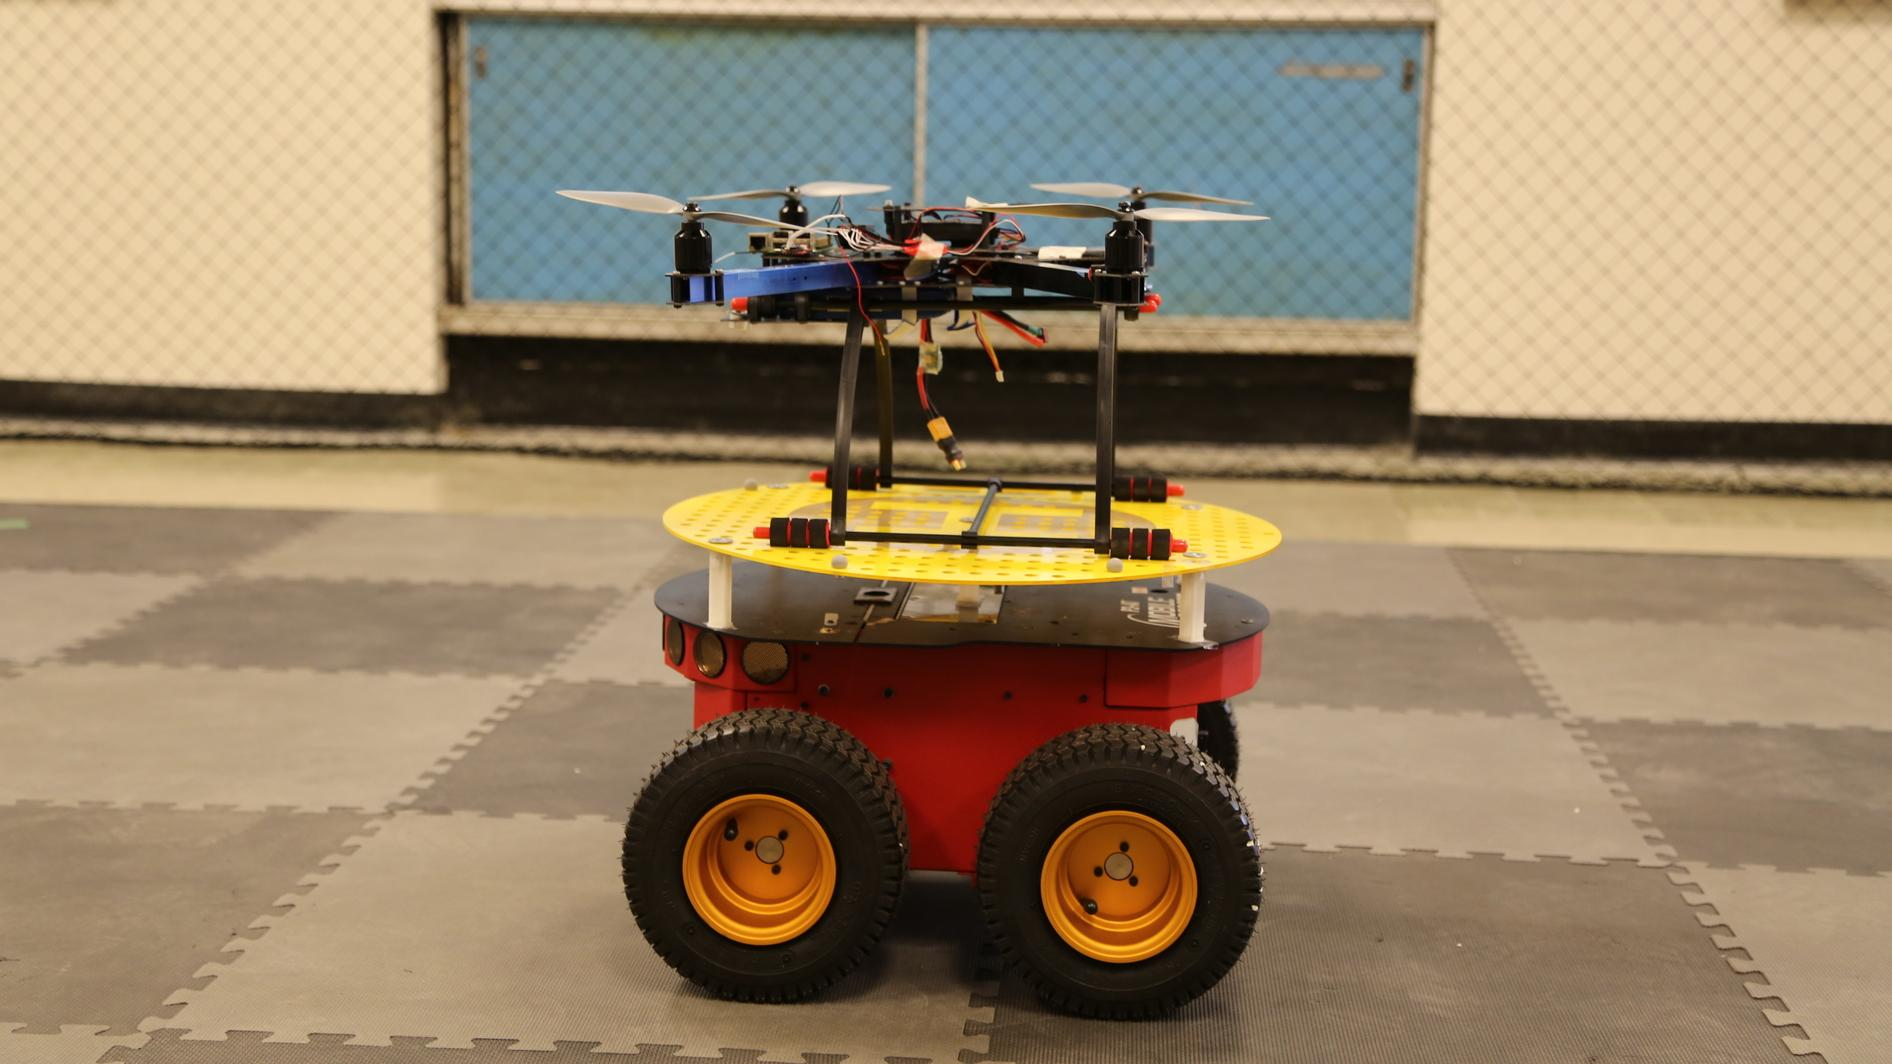
\includegraphics[width=0.6\textwidth]{images/irols.jpg}
    \caption{The test sUAV with the mobile target platform.}\label{f:lezl-olli}
\end{figure}

\subsection{Onboard Software}
ROS is an open source framework developed specifically to ease the development of software for robotics and
robotics control\cite{quigley2009ros}. Using ROS, it becomes a simple task to distribute computational loads
across a computational graph of separate nodes. Additionally, ROS has a rich library of packages which are
both useful for low-level processing of sensor information or managing hardware interfaces, and also
high-level behavioral control or localization schemes. This project relies heavily on the work of many others
in the area of visual odometry\cite{olson2011tags}, kalman filtering\cite{MooreStouchKeneralizedEkf2014}, and
flight control\cite{rotors:2016,meier2015px4}. The structure allows a roboticist to build and manage highly
complex systems in a reliable way (see \cref{f:rosgraph}

\begin{figure}[ht]
    \centering
    \includedot[angle=90,scale=0.2]{tikz/rosgraph}
    \caption{Sample compute graph for a single mission simulation. Note that each node in the graph represents
    a computational unit. The edges between nodes represent data sharing}\label{f:rosgraph}
\end{figure}

Control of the quadcopter is handled in discrete stages based on vehicle state. It is assumed that the vehicle
will have a rough estimate of the target location given to it so that it can travel to the appropriate region
and find the target in the field of view of the camera sensor. Vehicle motion from arming until target
location is handled by sending waypoints to the flight controller. Once the target is located in the image,
The vehicle gives control over to a set of FISs. The controller is described in more detail in
\cref{s:landing:controller}. The vehicle behavior over an entire mission is handled using a state
machine\cite{bohren2010smach}. Using a state machine allows the control to be handled in well-defined domains
and ensures that transitions between states are handled smoothly. The states comprising a full mission from
take to landing are shown in \cref{f:smach}.

\begin{figure}[ht]
    \centering
    \includedot[scale=0.5]{tikz/smach}
    \caption{State machine of robotic lander}\label{f:smach}
\end{figure}

The state of the vehicle is managed by fusing together the positional estimate from the camera sensor and the
AprilTag estimate (see \cref{s:landing:cv} as well as orientation information from the onboard IMU using an
extended kalman filter (EKF). This estimate is only valid when the vehicle has a visual track on the target
platform, otherwise, it is assumed that the vehicle is still in transit from its launch location, or it has
landed. As can be seen in \cref{f:smach}, the mission starts by arming the vehicle and immiediately sending
the waypoint to approach the target area. When the vehicle enters the ``TRACK'' state, it is en route to the
target location; while in this state, it monitors the quality of its visual estimation of the target location
by evaluating the norm of the covariance matrix computed by the EKF. Only when the covariance is sufficently
small does the vehicle transition to the next state.

The transition to the ``APPROACH\_LAND'' state signals the transfer of control from the flight controller's
waypoint manager to the FISs. While the vehicle is approaching and eventually landing on the target pad, a
wrapping state monitors the state of the vehicle to calculate a fitness of the behavior. This fitness is
returned to a master process which manages individual runs to execute the GA. In actual flight on hardware,
the fitness process would be absent. When the vehicle meets a proximity threshold in the ``APPROACH'' state,
it transitions to the ``LAND'' state and puts down onto the landing pad. The details of the simulation,
control, vision estimation, and devlopment process are discussed at length in the following sections.

\section{Simulation}
Gazebo is a 3D simulation software which uses open source dynamics engines Bullet, Dart, and ODE to model its
components. While Gazebo has very high fidelity simulation capabilities for robots (its initial purpose), the
complexities of aerodynamics in general, and multicopter physics in particular, can only be modeled with many
simplifications. Even with the simplified dynamics, the simulation environment that Gazebo provides is very
useful for high-level controller development. Gazebo allows for the simulation of many sensor types and nicely
integrates with ROS and the PX4 flight controller firmware. The high fidelity of the simulation will ease the
transition from virtual to real flight as all hardware components have simulated counterparts. The simulation
provides a real time interface for tuning the controller with visual feedback. This is the process which was
used to tune the PID controller and will be used as well for the tuning of the fuzzy controller.

The most important aspect of sensing for the system is the image sensor. A camera sensor is simulated from the
underside of the quadrotor to test the efficacy and efficiency of the computer vision algorithms. Care was
taken to accurately represent the field of view and pixel noise of the physical camera sensor to be used. In
this way, it is hoped that the controllers developed in simulation will be applicable on the physical system.

The high fidelity of the simulation comes with the drawback that it is only able to be run in real time,
making training with a GA difficult to attain in any reasonable amount of time. Another drawback of accuracy
is that simulation is that each individual sensor in the simulation is modeled with near-realistic noise
values. This is by design in order to train a robust controller, but comes with the side effect that no
simulation run is perfectly repeatable. This introduces the frequent case that the top-performing controller
from on GA generation may be a failure on the next due to either it being overtrained, or a case of bad luck.
For this reason, the GA was never ver successful at training a controller which performed well consistently.
In the end, a fuzzy controller was hand-tuned to meet the needs of the controller. Although the GA was never
successful, much important information was gained in the process of making the attempt.

\subsection{Fitness Function Development} The author was met with surprising difficulty in developing an
effective cost function. Most attempts resulted in unintended consequences with minima resulting from
non-optimal behavior. Finally the fitness function was broken into a behavioral fitness function (BFF) (
\cref{e:bff}) to grade the action of the vehicle over time and an aggregate fitness function (AFF) (
\cref{e:aff}) to measure the fitness of the final state of the vehicle. These are linearly combined to create
a tailored fitness function (TFF)\cite{divband2015effect}.

\begin{align}
J_{bff} &= \sum_{i=0}\left(\hat{p}_i\cdot\hat{v}_i + 1\right)\frac{t_i}{|t|} \label{e:bff}\\
    J_{aff} &= |p_f| \label{e:aff}\\
    J_{tff} &= J_{bff}J_{tff}\label{e:ff}
\end{align}
where $\hat{p}$ is the unit position vector of the vehicle with respect to the landing pad, $\hat{v}$ is the
unit velocity vector, and the subscript $i$ denotes a single instant in the time history. Note that the time
must be normalized because the time taken for a full simulation from target track to landing will take a
non-deterministic time. This scaling by the time step serves the function of penalizing late-game mistakes
greater than early errors; errors in the terminal stage of approach are more likely to abort the process, so
require a stricter grading. This time-scaling requires that the BFF be computed post-facto as opposed to in
real time.

\section{Controller}\label{s:landing:controller}
Control is exerted on the vehicle by supplying the flight controller with changes in the velocities, $\Delta
v_x$, $\Delta v_y$, and $\Delta v_z$, as well as yaw rate, $\dot{\psi}$. The quadrotor is able to land with
any arbitrary yaw angle, $\psi$, but the assumption is made that some reception mechanism may expect the
vehicle in a nose-forward orientation. Distance to the platform is estimated from images taken by the camera
sensor. Orientation is estimated only in the last phase of the landing sequence using a robust and efficient
visual fiducial tag system\cite{olson2011tags} (see \cref{f:apriltag}).
\nomenclature[]{$\Delta v_x$}{Control input change to velocity in $x$-axis}
\nomenclature[]{$\Delta v_y$}{Control input change to velocity in $y$-axis}
\nomenclature[]{$\Delta v_z$}{Control input change to velocity in $z$-axis}
\nomenclature[]{$\dot{\psi}$}{Control input to yaw rate (rotation about $z$-axis)}

\subsection{Computer Vision}\label{s:landing:cv}
Much emphasis is put on the sensing algorithms to be computationally efficient to decrease the load on the
on-board computer. For this purpose, only a small number of image processes are required to detect and locate
the target. As a first pass, the image is brought into the Hue-Saturation-Value (HSV) color space. This has
been shown to be a robust space in which do perform color detection and segmentation in uncontrolled and
unpredictable lighting conditions\cite{zhao2002robust}. A simple thresholding is performed on the image to
isolate a sufficiently wide band of yellows to match the color of the target and dilate this to a binary blob.
From this binary image, the image moments are calculated by
\begin{figure}[ht]
    \centering
    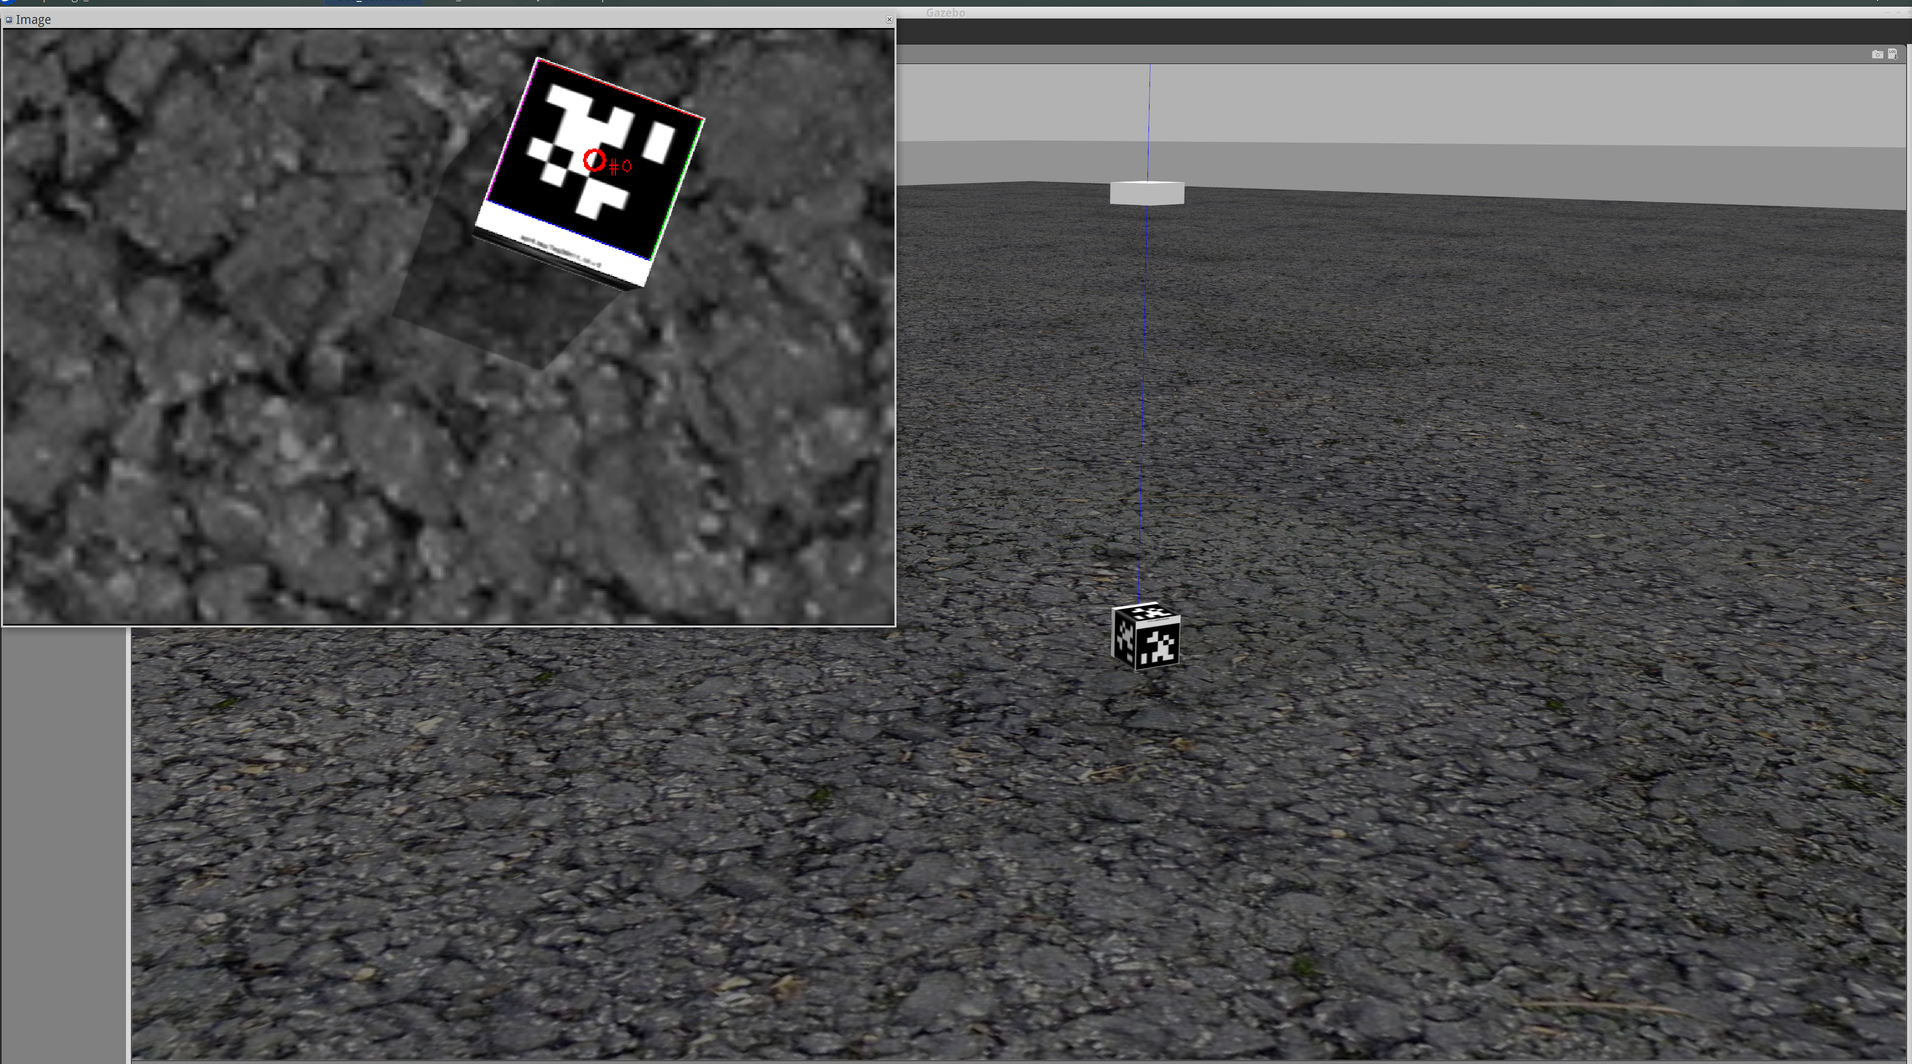
\includegraphics[width=0.8\textwidth]{images/rs_working_apriltags_crop.png}
    \caption{Simulated image sensor detection of AprilTag marker.}\label{f:apriltag}
\end{figure}

\begin{equation}\label{e:im_moments}
    m_{ij}=\sum_{x,y}x^iy^jI_{xy}
\end{equation}
\nomenclature[]{$m_{ij}$}{Raw image moment}
\nomenclature[]{$I_{xy}$}{Pixel intensity value}
where $I_{xy}$ is the pixel intensity value for each pixel $(x,y)$ (equal to 1 in this case) and $i,j =
0,1,2$. From this it can be seen that $m_{00}$ describes the area and $\frac{m_{10}}{m_{00}}$ and
$\frac{m_{01}}{m_{00}}$ describe the centroids $\overline{x}_p$ and $\overline{y}_p$ in terms of pixels. The
blob is assumed to be circular and hence a diameter is extracted from the pixel area. Using the focal length
of the sensor, these image points are then projected onto the ground plane using the known diameter of the
landing pad and a vertical offset estimate is obtained as is shown in \cref{e:dist_est}.
\begin{equation}\label{e:dist_est}
    d_z=\frac{d\cdot f}{m\cdot d_p}
\end{equation}
where $f$ is the focal length of the camera in units of length, $d$ is the known diameter of the landing pad,
$d_p$ is the estimated diameter in pixels, and $m$ represents a scaling factor in units of \si{\px\per\mm}
(unity in the simulation).
\nomenclature[]{$f$}{Focal length of image sensor}
\nomenclature[]{$m$}{Pixel scaling factor}
Assuming that the image plane and the ground plane are parallel, the center of the image can be assumed to
point directly below the vehicle and the horizontal offsets to the landing pad can then be calculated as
\begin{align}\label{e:horiz_est}
    d_x &= d_z\cdot\frac{m\overline{x}_p}{f}\\
    d_y &= d_z\cdot\frac{m\overline{y}_p}{f}
\end{align}
\nomenclature[]{$d_x$}{Horizontal offset error from vehicle to target in the body-fixed $x$-axis}
\nomenclature[]{$d_y$}{Horizontal offset error from vehicle to target in the body-fixed $y$-axis}
\nomenclature[]{$d_z$}{Vertical offset error from vehicle to the target}

As the vehicle approaches the landing pad, the image field of view is overtaken by the landing pad itself and
the former segmentation no longer becomes effective. For this purpose, an apriltag\cite{olson2011tags} (see
\cref{f:apriltag}) is placed on the center of the target. Once detection of this tag is achieved, an refined
estimate of position and even orientation is obtained with respect to the target. This estimate is used to
then orient the vehicle to match the heading of the landing pad (see \cref{f:landing_ims}).

\begin{figure}
    \begin{subfigmatrix}{4}% number of columns
        \subfigure[\label{f:colora}]{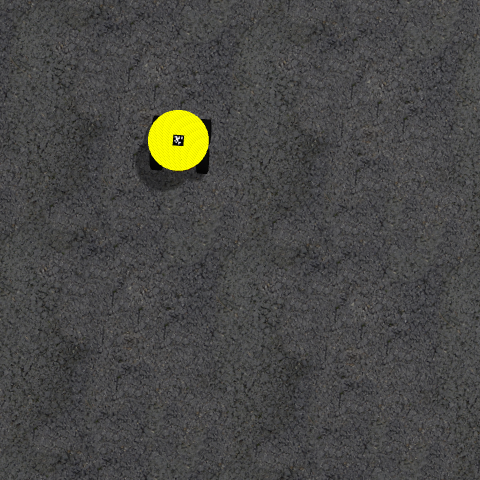
\includegraphics[width=0.2\textwidth]{images/image1_18469000.png}}
        \subfigure[]{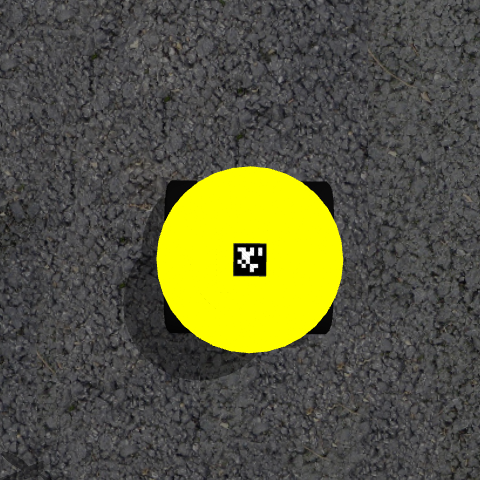
\includegraphics[width=0.2\textwidth]{images/image1_30863000.png}}
        \subfigure[]{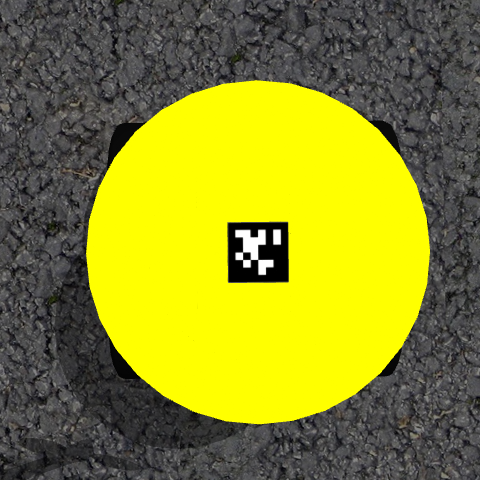
\includegraphics[width=0.2\textwidth]{images/image1_36074000.png}}
        \subfigure[\label{f:colorb}]{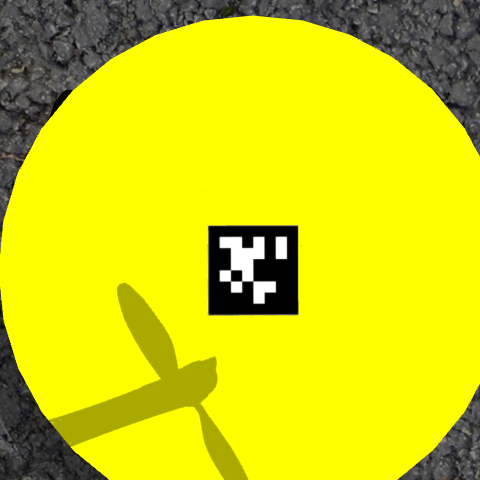
\includegraphics[width=0.2\textwidth]{images/image1_38233000.png}}
        \subfigure[\label{f:aprila}]{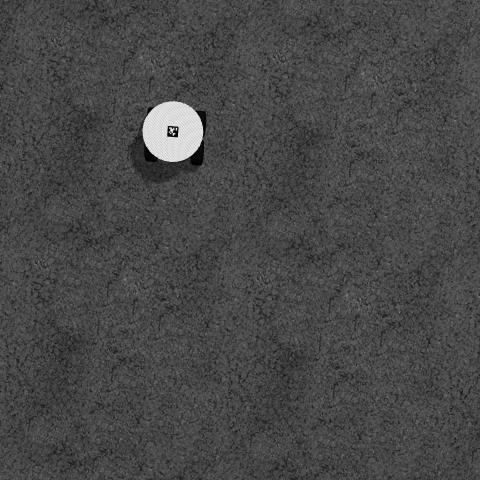
\includegraphics[width=0.2\textwidth]{images/image2_18469000.png}}
        \subfigure[]{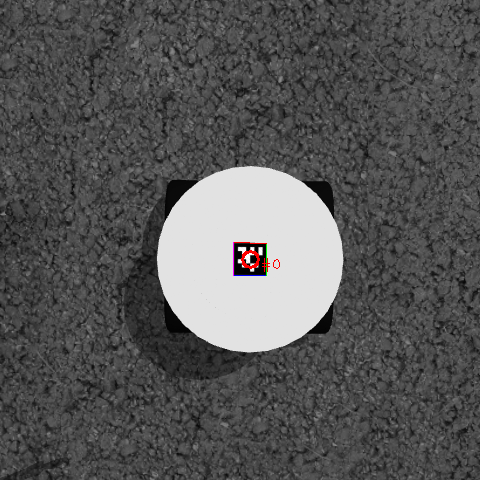
\includegraphics[width=0.2\textwidth]{images/image2_30863000.png}}
        \subfigure[]{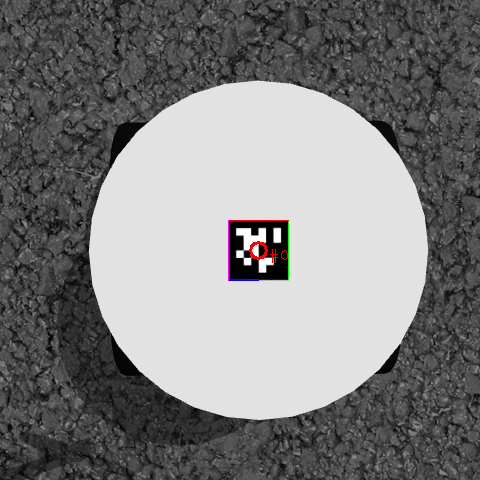
\includegraphics[width=0.2\textwidth]{images/image2_36074000.png}}
        \subfigure[\label{f:aprilb}]{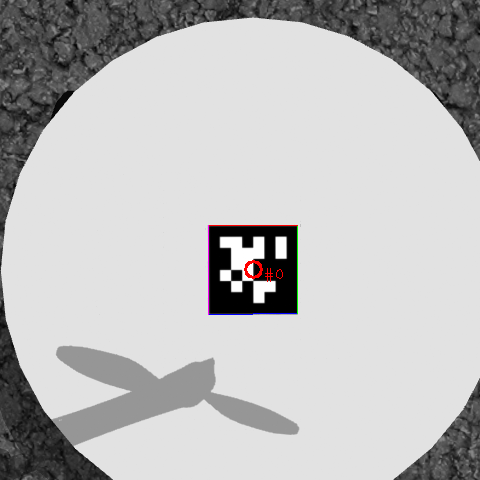
\includegraphics[width=0.2\textwidth]{images/image2_38233000.png}}
        \subfigure[\label{f:cva}]{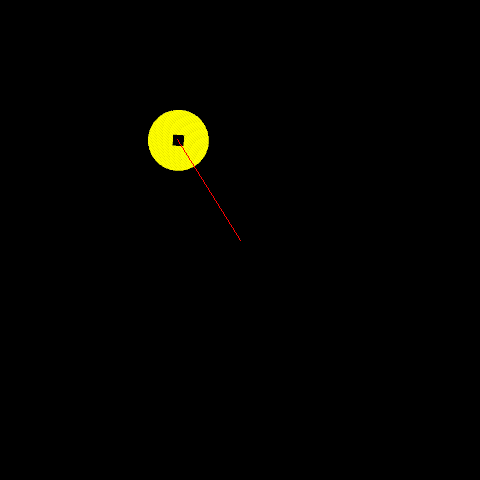
\includegraphics[width=0.2\textwidth]{images/image1_18469000_proc.png}}
        \subfigure[]{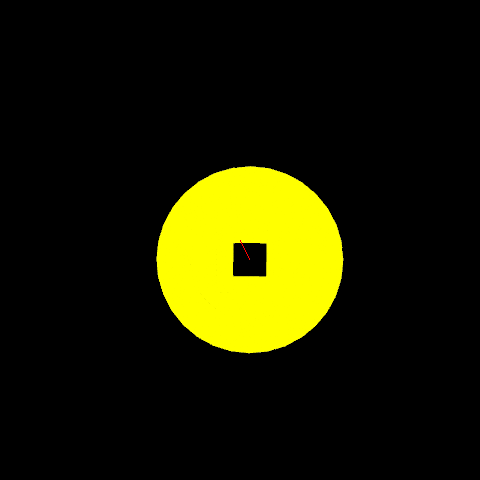
\includegraphics[width=0.2\textwidth]{images/image1_30863000_proc.png}}
        \subfigure[]{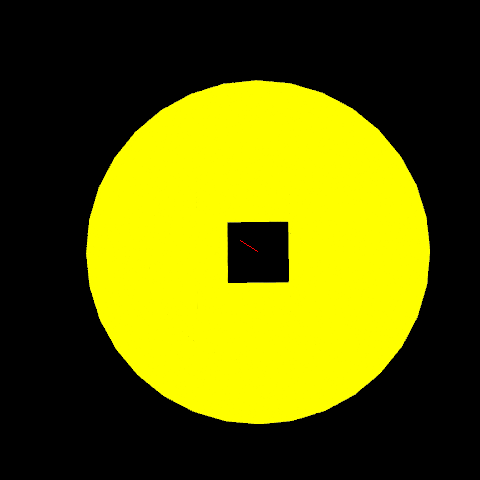
\includegraphics[width=0.2\textwidth]{images/image1_36074000_proc.png}}
        \subfigure[\label{f:cvb}]{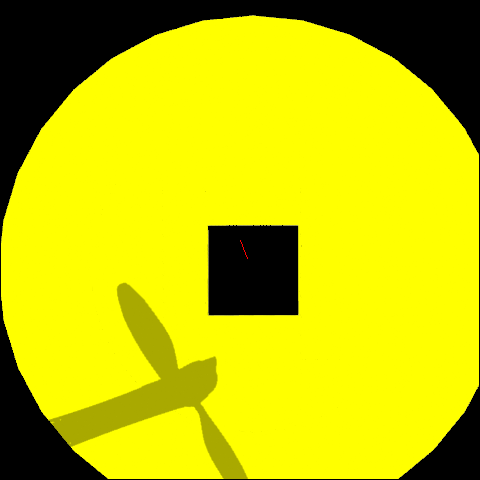
\includegraphics[width=0.2\textwidth]{images/image1_38233000_proc.png}}
    \end{subfigmatrix}
    \caption{A time series of images taken during the landing maneuver. Note that in \cref{f:aprila}, there is
    no detection of the marker and there remains a slight error in yaw angle as a result. The red line in
\crefrange{f:cva}{f:cvb} represents the horizontal offset of the vehicle to the desired point on the target.}
    \label{f:landing_ims}
\end{figure}

\subsection{PID Results}
A PID controller was created which uses the most recent error estimates and sends velocity requests to the
flight controller. Due to the lack of a mathematical model of the system. The PID gains were found by
iterating the simulation with various position setpoints and dynamically adjusting the gains while observing
the response visually. This closely mimics the method by which PID gains are attained in the tuning of an
actual quadrotor by flying a series of test flights and adjusting gain values by feel. In this way, a
reasonable response and landing sequence was achieved for first a static target and then repeated for a
dynamic target moving with constant velocity. The results are presented in \crefrange{f:pid_stat}{f:pid_dyn}
in which the normed horizontal offset from target is shown in conjunction with the vertical distance to the
platform. Viewing the charts, it is apparent that as the vehicle approaches the target, it tends to accumulate
horizontal errors and must correct more frequently, particularly in the dynamic case. In both cases, the
quadrotor managed to successfully land on the target. In the static case, the final offset from the center of
the target was less than \SI{5}{\cm}. For the dynamic case, the error was \SI{7}{\cm} which nearly displaced
it from the target surface. In both cases, the sink rate and yaw rates were controlled by simple PD
controllers.



\subsection{Fuzzy Results}
Though this work is still in progress, promising preliminary results in development of a fuzzy controller have
been obtained. Four fuzzy controllers of similar architecture were created as shown in \cref{f:fuzzy_mfs}.
Each input fuzzy partition was multiplied by a scaling factor to bring it into the regime of the controller.
Likewise, the outputs were then again scaled to match actuation limits. The rule base was developed using
common intuition about the system dynamics. A full rule matrix was defined to fully cover the system
possibilities. This rule matrix is shown in \cref{t:rules}. The rules are made up of linguistic variables
composed into IF-THEN constructions of antecedents and consequents. For example:
\begin{center}
    IF \emph{error} is \textbf{N} AND \emph{error rate} is \textbf{Z} THEN \emph{$\Delta v$} is \textbf{SP}
\end{center}

\begin{figure}[h]
    \begin{subfigmatrix}{3}
        \subfigure[Fuzzy input partition template\label{f:error_in_mfs}]{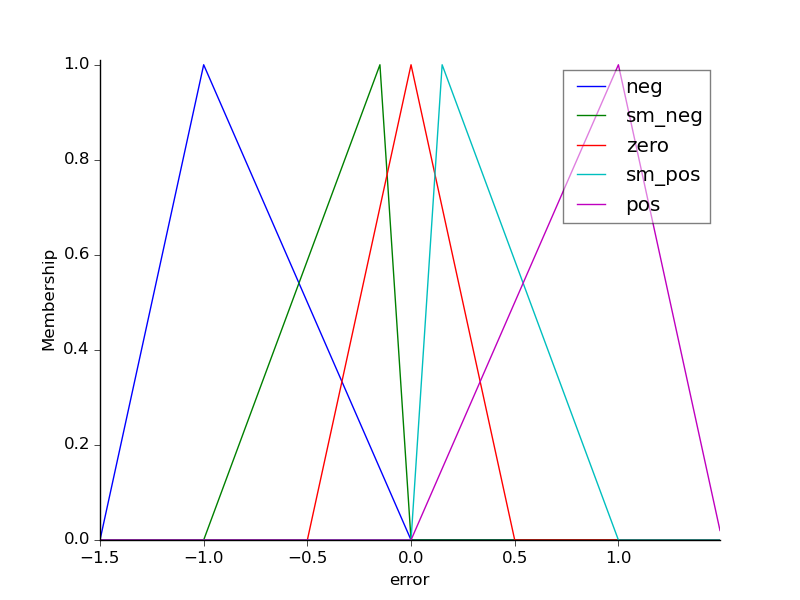
\includegraphics{images/error_in.png}}
        \subfigure[Fuzzy input partition template\label{f:error_d_in_mfs}]{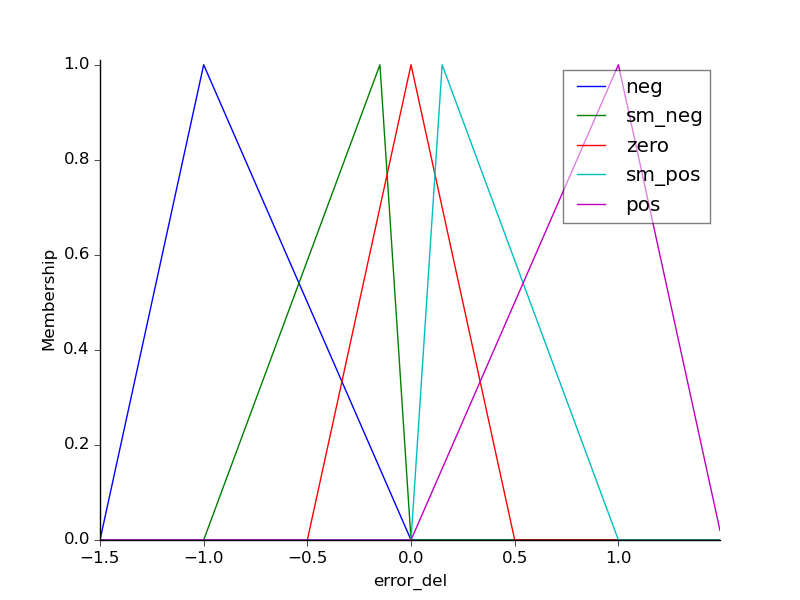
\includegraphics{images/error_del_in.png}}
        \subfigure[Fuzzy output partition template\label{f:vel_out_mfs}]{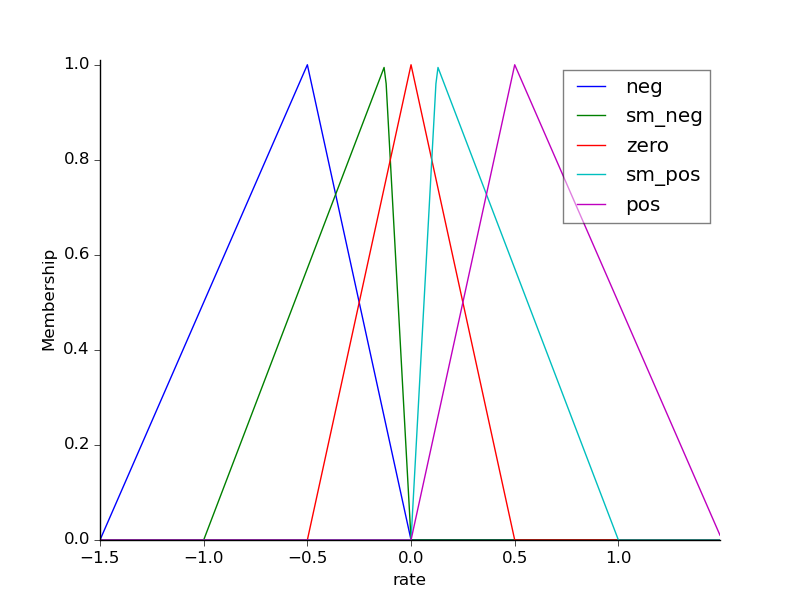
\includegraphics{images/vel_out.png}}
    \end{subfigmatrix}
    \caption{Membership function definitions for fuzzy logic controller.}\label{f:fuzzy_mfs}
\end{figure}
These rules are intuitive and easy to understand and provide a process by which to lend the controller a
decision-making system with a foundation in human reasoning. The tuning process of the fuzzy controller then
becomes the task of defining the membership functions which decide how much of each rule should be activated
for certain inputs. Triangular membership functions are used exclusively for their simplicity in definition
and tuning\cite{mishra1994performance} while the aggregation of rules is the popular min-max method put forth
by Mamdani\cite{MAMDANI19751}. The membership functions shown in \cref{f:fuzzy_mfs} are the result of only a
small number of iterative tuning steps and were found to be the most effective of the configurations
attempted. The fuzzy rule base also provides ample opportunities for tuning and will have a significant impact
on controller performance.


\begin{table}[ht]
    \centering
    \caption{Fuzzy rule base}\label{t:rules}
    \begin{tabular}{cc||c|c|c|c|c|}
        &  \multicolumn{6}{c}{error}  \\ 	
        \multirow{6}{*}{error rate} &    & N  & SN & Z  & SP & P  \\ 	\hhline{~=#=|=|=|=|=|}
                                    & N  & P  & P  & SP & SP & Z  \\ 	\cline{2-7}
                                    & SN & P  & SP & SP & Z  & SN \\ 	\cline{2-7}
                                    & Z  & SP & SP & Z  & SN & SN \\ 	\cline{2-7}
                                    & SP & SP & Z  & SN & SN & N  \\ 	\cline{2-7}
                                    & P  & Z  & SN & SN & N  & N  \\ 	\cline{2-7}
    \end{tabular}
\end{table}

The result of this first-iteration controller was sufficient to land the quadrotor on both the static and
constant linear velocity dynamic platforms, though the response to uncertainties is not very stable as of yet.
The results shown in \crefrange{f:fuz_stat}{f:fuz_dyn} demonstrate the difficulty an untrained controller may
have with novel situations. The results are expected to improve dramatically by using genetic algorithms to
tune each controller.
\begin{figure}[h]
    \begin{subfigmatrix}{2}
        \subfigure[$(kp,ki,kd)=(2.1,0.015,0.2)$ for static target interception.\label{f:pid_stat}]{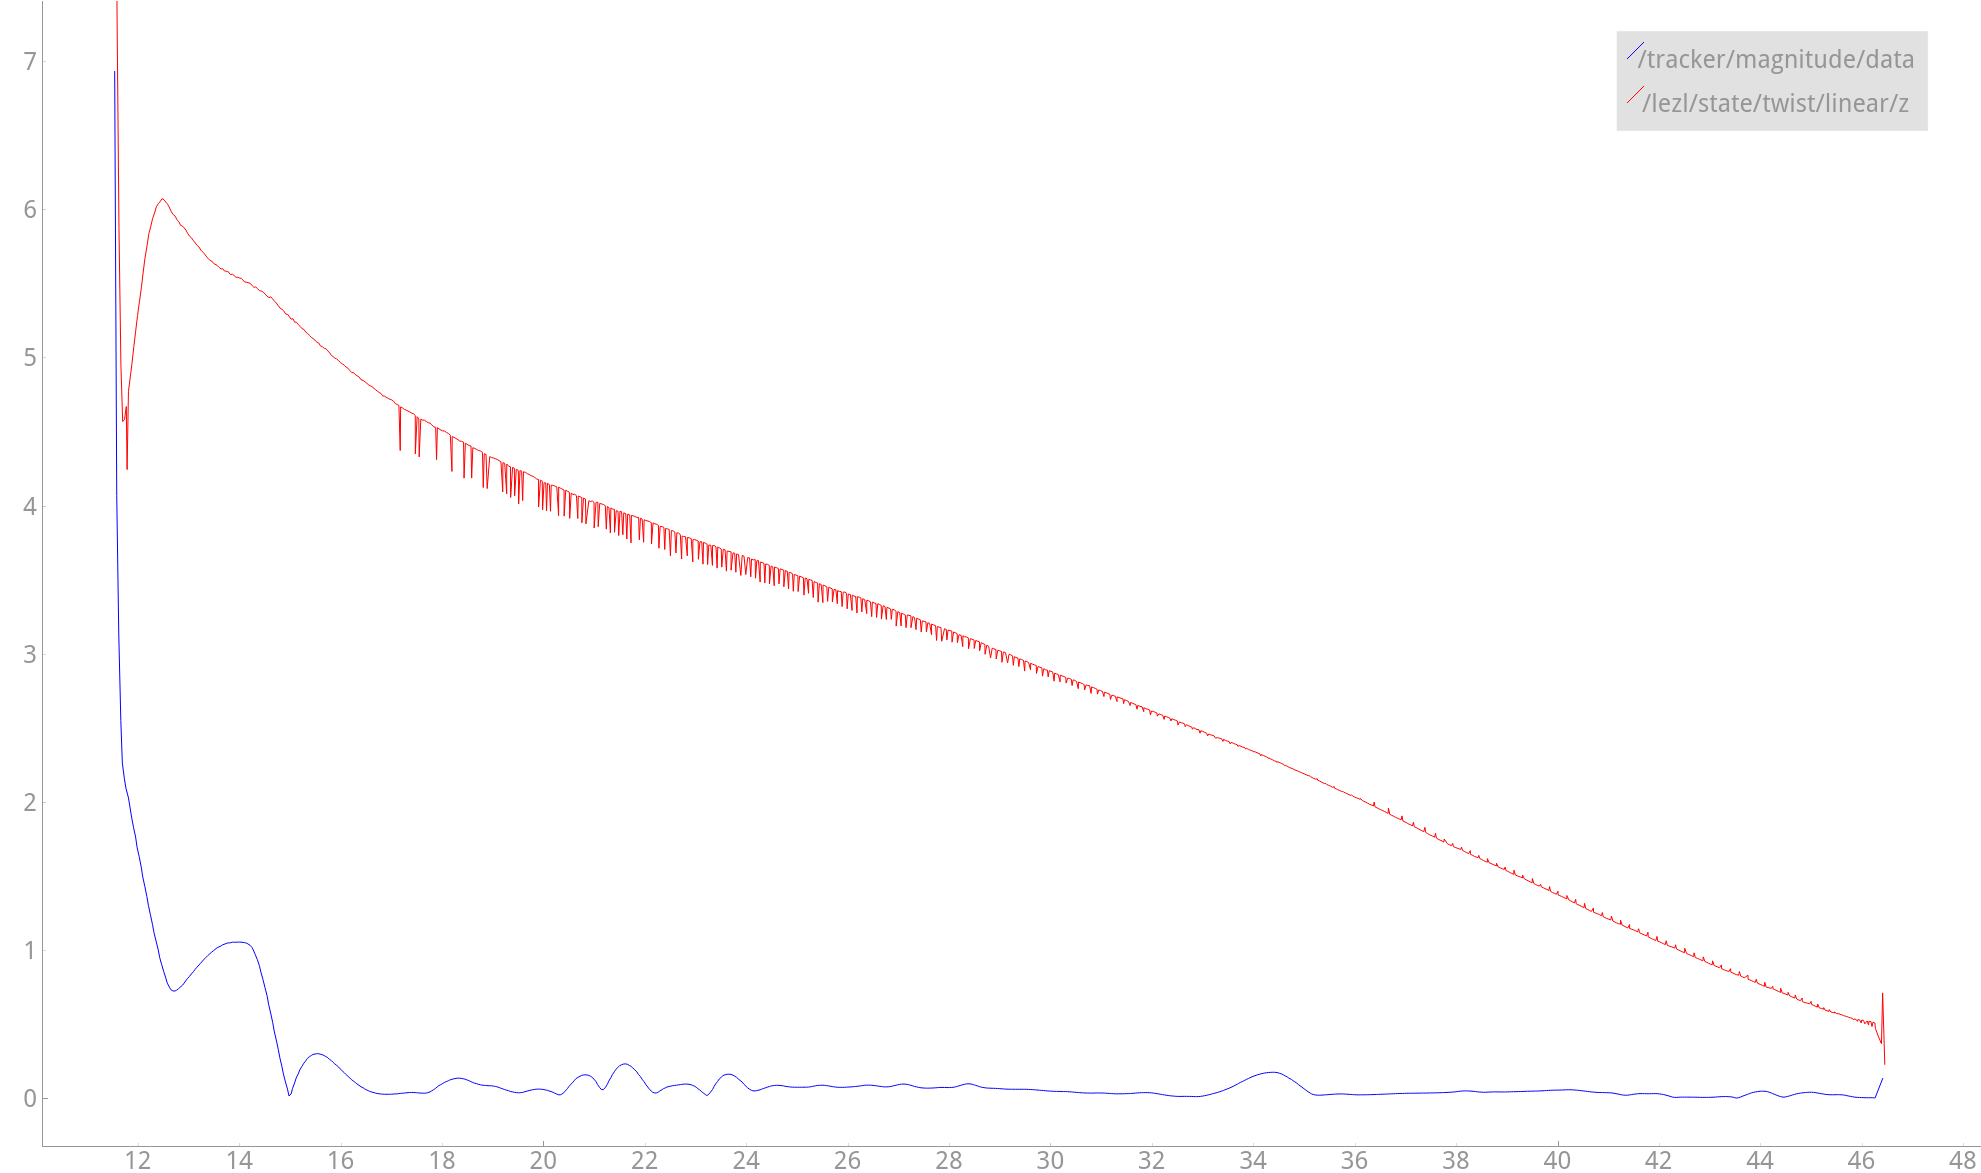
\includegraphics[width=0.45\textwidth]{images/mag_z_pid_static.png}}
        \subfigure[$(k_p,k_i,k_d)=(1.8,0.012,0.02)$ for dynamic target interception.\label{f:pid_dyn}]{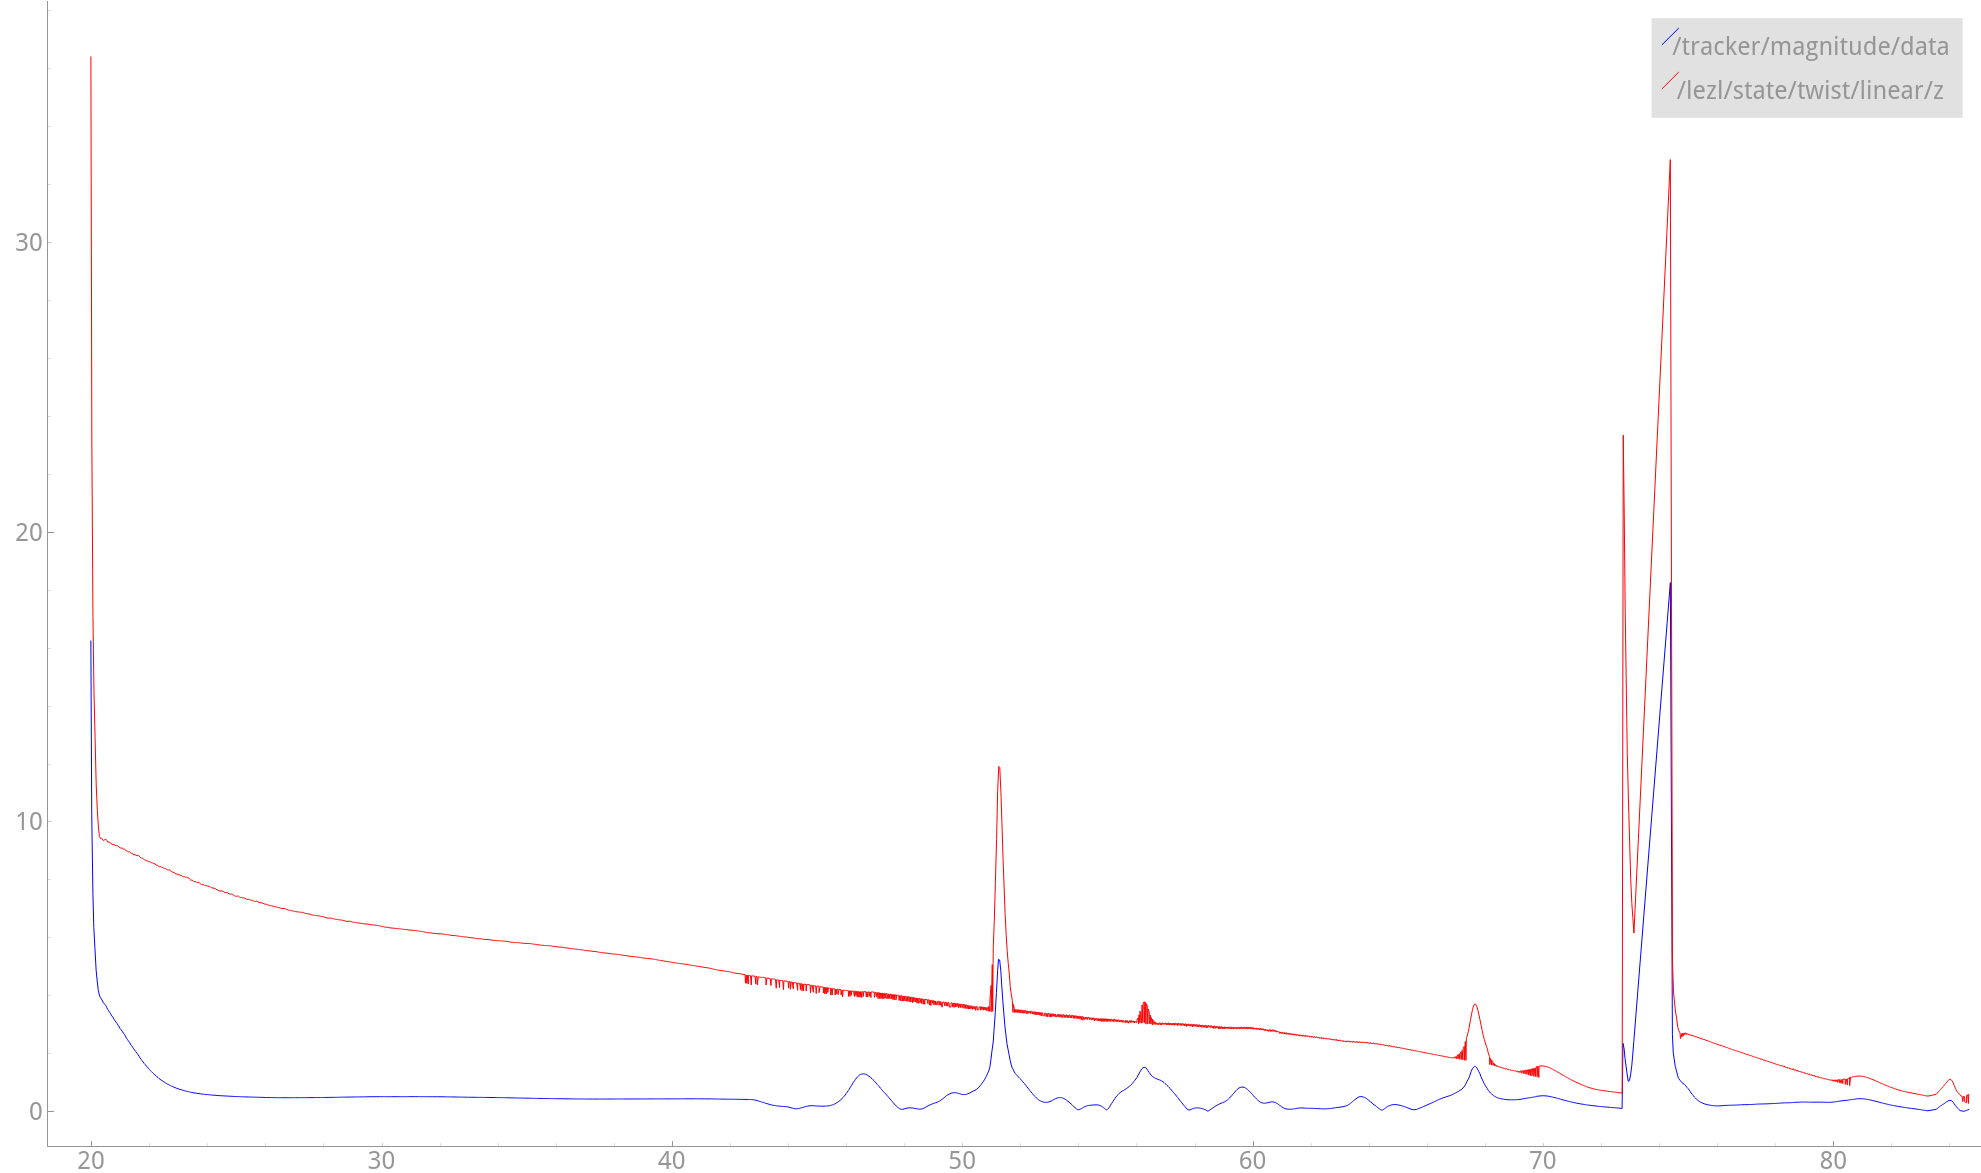
\includegraphics[width=0.45\textwidth]{images/mag_z_pid_dynamic.png}}
    \end{subfigmatrix}
    \caption{PID controllers for static and dynamic landing}\label{f:pid_lands}
\end{figure}
\begin{figure}[h]
    \begin{subfigmatrix}{2}
        \subfigure[Static target interception.\label{f:fuz_stat}]{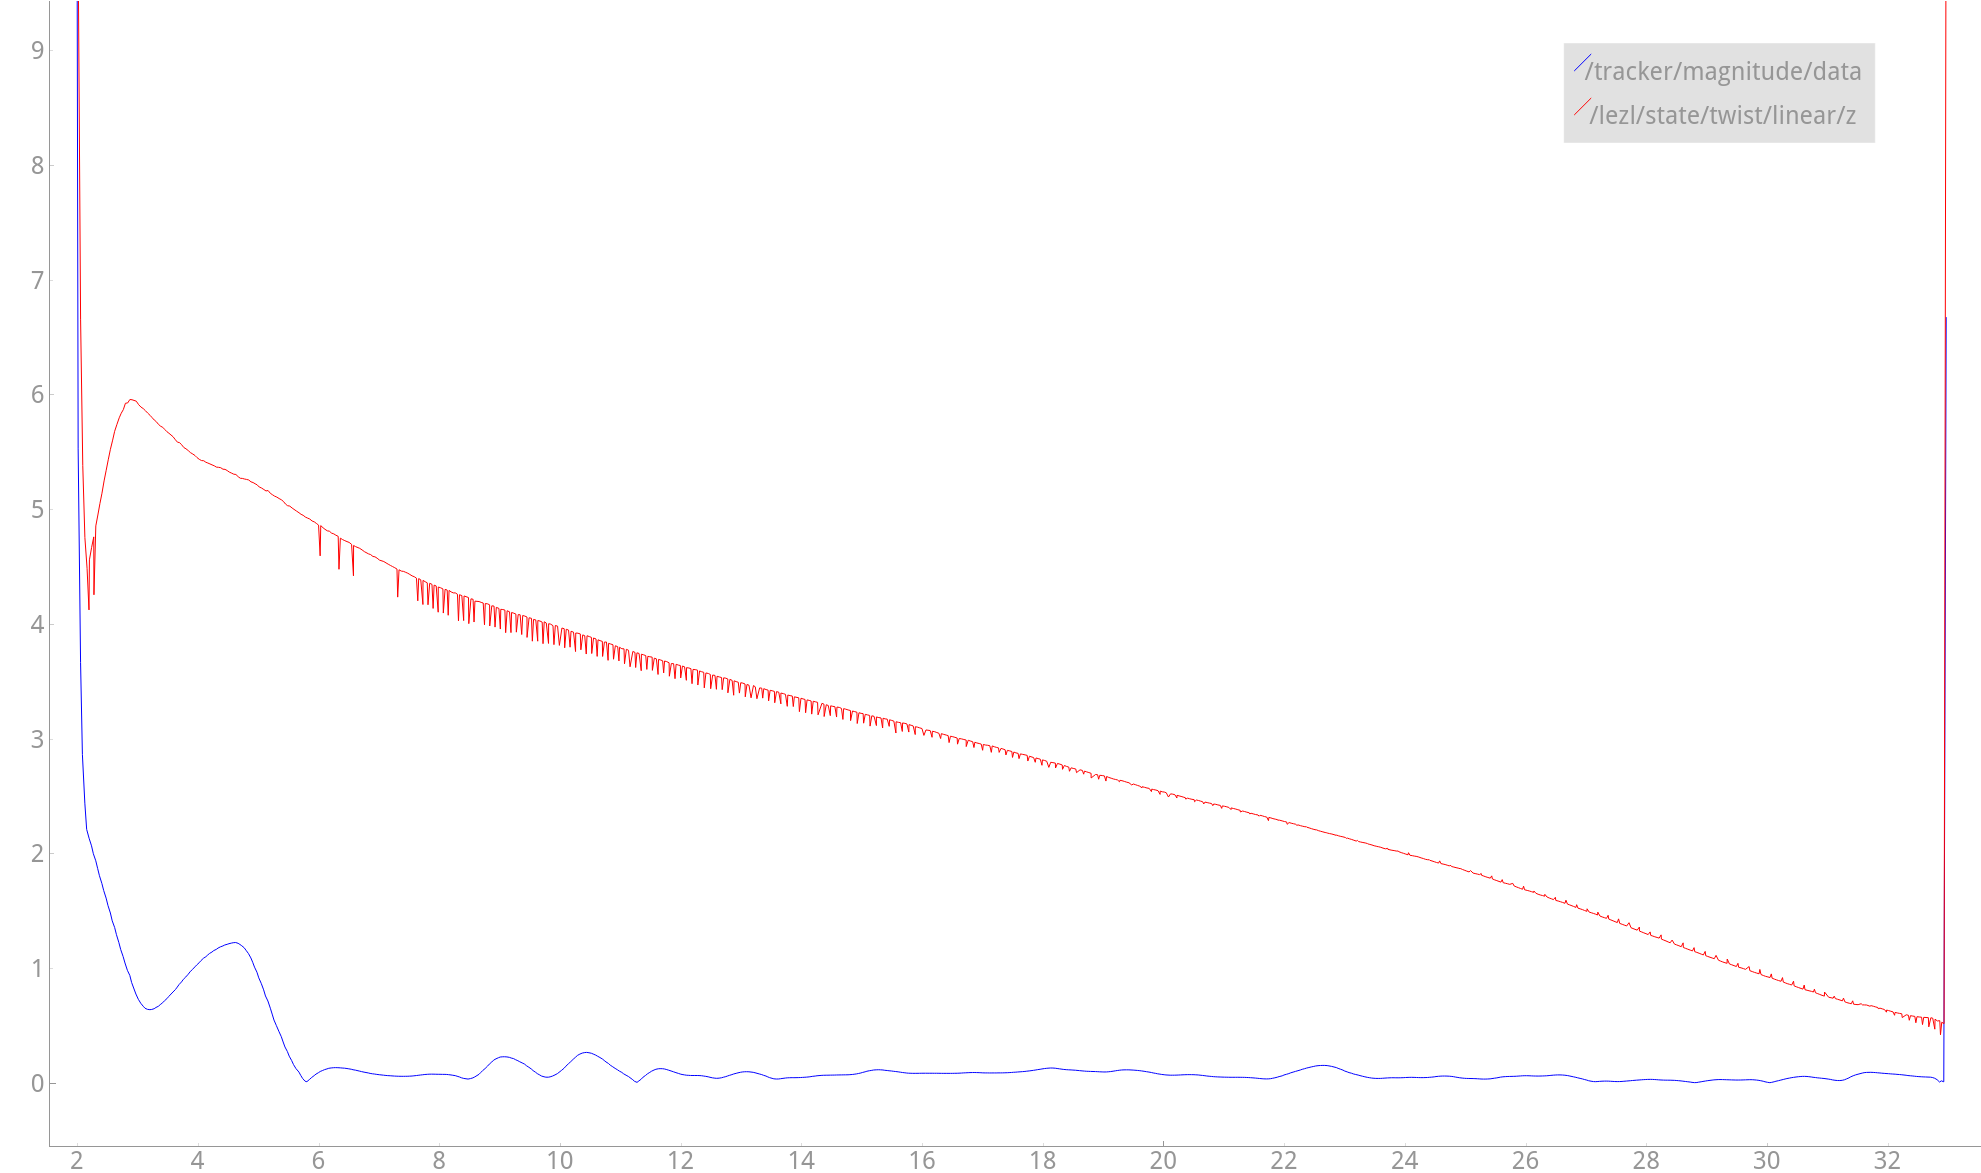
\includegraphics[width=0.45\textwidth]{images/mag_z_fuzzy_static3.png}}
        \subfigure[Dynamic target interception.\label{f:fuz_dyn}]{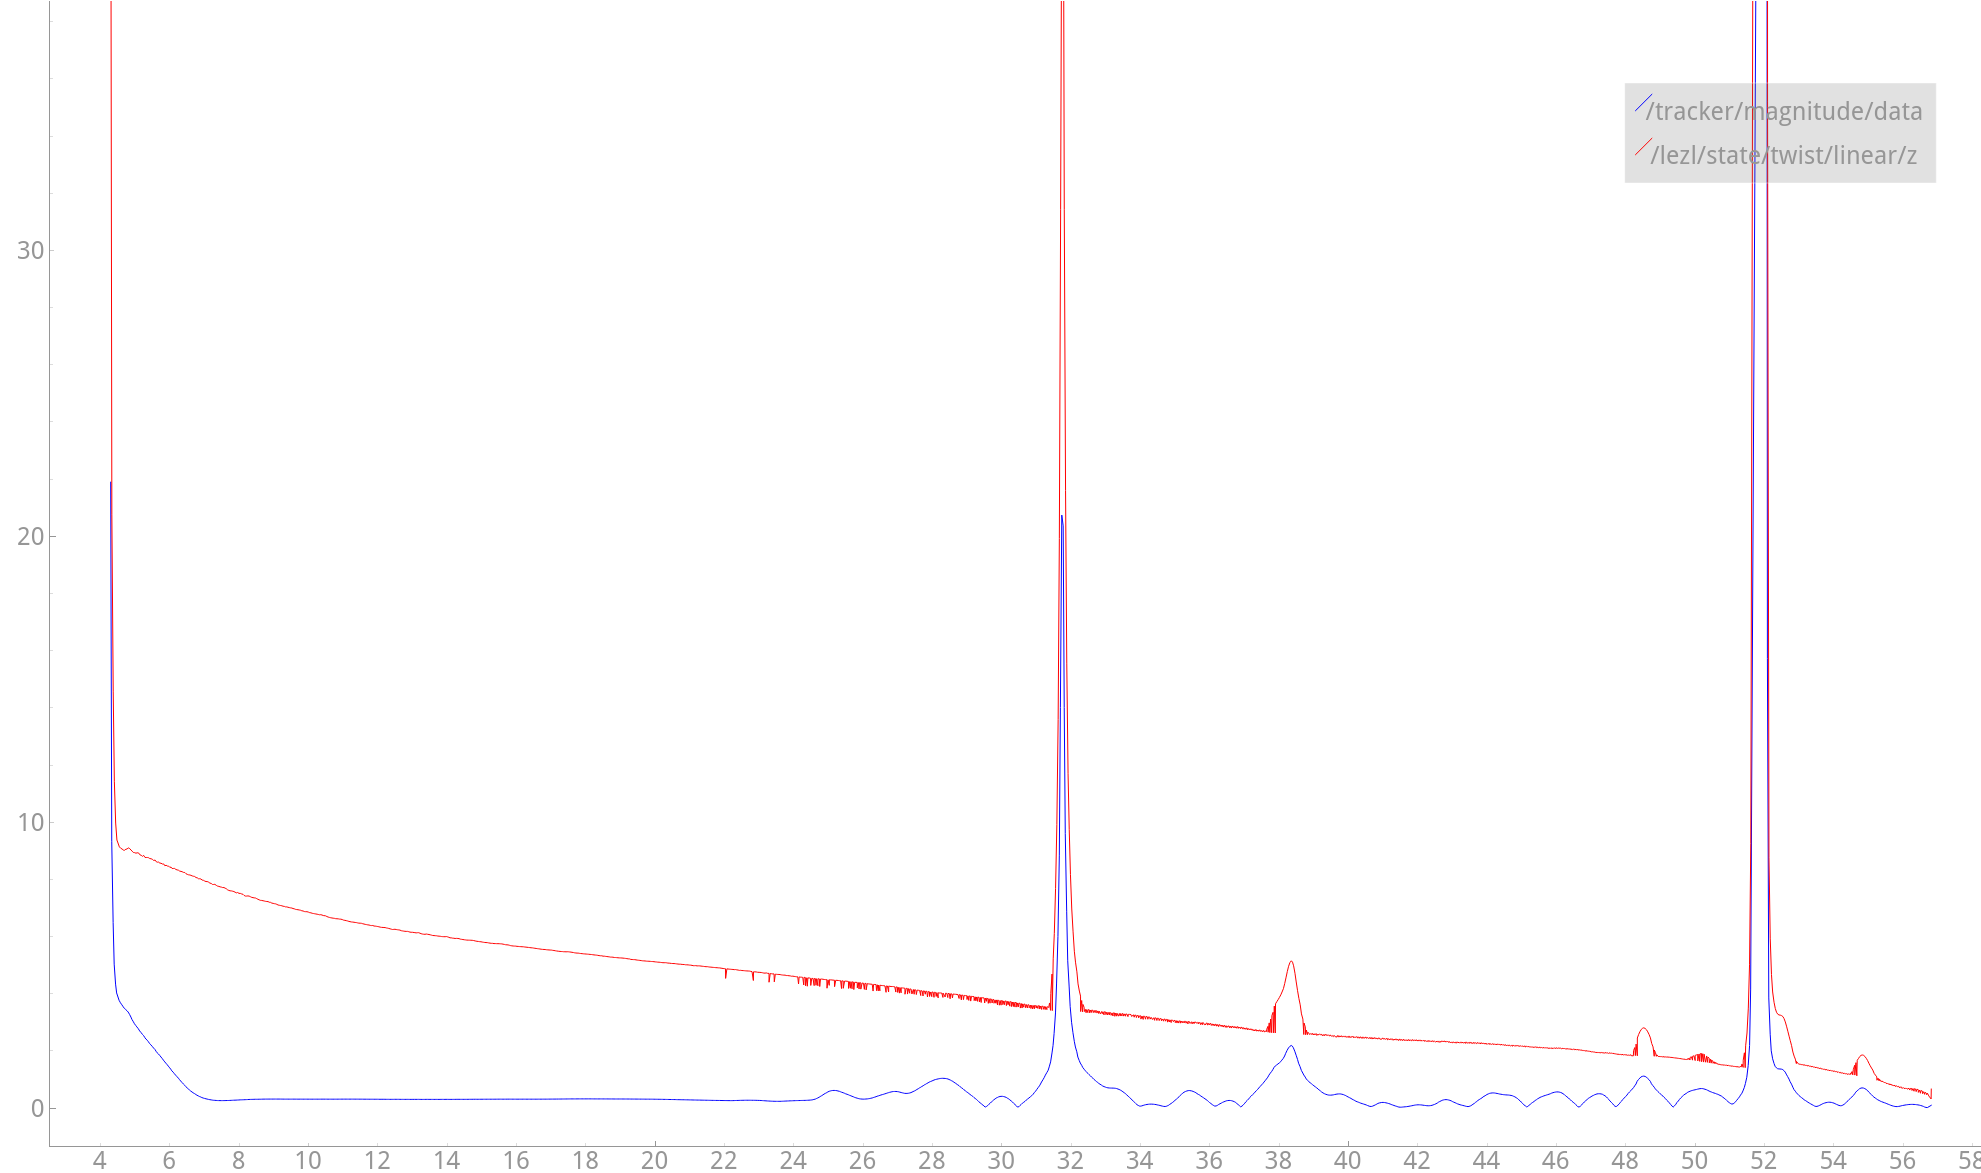
\includegraphics[width=0.45\textwidth]{images/mag_z_fuzzy_dynamic3.png}}
    \end{subfigmatrix}
    \caption{Fuzzy controllers for static and dynamic landing}\label{f:fuzzy_lands}
\end{figure}

\section{Conclusion}
The results presented are preliminary only, but show promising results. The control effort of the untuned
fuzzy controller nearly matched that of the tuned PID controller for the  static target case. For the dynamic
target, while neither controller was tuned to any high degree of accuracy, the fuzzy controller performed at
least as well as the PID controller. It should be noted that the overall positioning control of the
vehicle is relatively simple, but as it approaches more closely to the platform, small movements are
translated to larger apparent errors and the controller may make bad decisions. This explains the peaks which
can be seen in both of the dynamic situations; as the quadrotor becomes very near to the platform, it
occasionally loses visual sight of the key target and must then abort the landing and gain altitude to retry.

There is much future work to yet complete. Both the PID and Fuzzy controllers will be tuned by a genetic
algorithm which will greatly improve the performance of each. To prepare the system for real world
deployment, the perfect gimbal assumption being made in the simulation will be replaced with a rigidly mounted
camera. This will require then applying a rotational transform to each image pixel measurement which will
increase the uncertainty in each estimate. Finally, the image processing pipeline must be optimized even
further to decrease the computation load on the processor. With the current pipeline, the test hardware
processes images at around \SI{2}{\Hz}, which may introduce too much latency in the control feedback. Either
the image processing must be sped up, or the delay will need to be handled in some other fashion.

